\chapter{DevOps管理工具}
基本傳統開發工具到debug工具完,已經算是一個developer該了解與完成的工作了。但
軟體工程不光只是開發工具的使用,整組 team work 的管理工作是經理級以上人員也
需完成的,這在過去 build完測試後,與QA組或者公司對外的interface的資訊管理,
很多也必須自己寫工具寫自動化script,或者依靠大公司內部的工具支援組寫,但現在
opensource 也很多這種管理軟體,基本上這有很多,但比較通用的有 project managment
, document management, bug tracking (issue tracking), build automation, 
customer relationship mgmt (CRM), esclation等等,這會牽扯到很多不同組的協力工作
,包括開發,測試,PM, OPs, marketing 等等。以往這些工具都是散在很多地方,現在
要把他們整合就要有非常 knowledgable 的人, 新的開發文化引進了 deployment 的工作
, 也就是 operation, 所以全部放在一起的叫DevOps。
\\\\
由於整個DevOps其實要知道所有的流程管理,以前我們很多都是公司IT, tool 開發組
做的, 但是這些工具現在很多都是opensource做掉,公司的IT, tool 人員,反而只要負責
這些管理軟體的安裝,整合,維護,自動化等工作,往往這就是新的DevOps的工作。傳統
公司IT人員通常了解的是 OS, networking, storage, security等分類,例如有的非常
了解網路設備 cisco/juniper siwtch, VLAN, traffic設定,有的非常了解storgae設備
ibm, emc, netapp, filesystem, nfs設定等等,而DevOps除了這些基本要了解外,例如
要設定工具的使用權限,你一定要知道windows, linux上的使用者,LDAP, Radius等與網
路安全 ,NFS 網路檔案系統,才有辦法建制這些更上層的工具設定。
\\\\
DevOps 工作也有其toolchain,但是著眼於high level 管理軟體的整合,例如他們講
code時,不是指真的一行行的c, python,而是指coding時所需工具,例如前面所說的
gcc, SRM, code review, dynamic analysis等工具的了解與建制,在講build時,是指多
個build的狀態,build 時間長短等build process的管理,以此類推,但像 github,
bitbucket 這些工具後端有些自動化 script 要寫要維護也是需要寫 code。
\\\\
目前DevOps 的 toolchain 範例
\begin{itemize}
  \item code - gcc, svn, git, java, coverity, purify, valgraind...
  \item build - make, maven, ant, jenkins
  \item test - sonarQube
  \item package - artifact, jfrog
  \item release - github, project, release, download mgmt
  \item configure - docker, coreOS
  \item monitor - user experience, customer relationship
\end{itemize}
有的工具其實跨好多領域,例如github,同時可以做code 管理,release管理等等。有的
project management管理軟體同時含有bug tracking, monitoring等功能。所以也不是分
的那麼清楚,總之做這些工具的整合人員為DevOps,由於這裏面東西太多了,有些很基本
名詞,應該是要進這領域前就都該會的。

\section{project management}
  軟體工程指的是軟體從無到有生產所需的管理原則與理論,什麼waterfall啦,spiral啦
  。後來還有 extreme programming 也被炒作啦,現在炒最凶的的就是agile啦。但管理
  跟其他工具一樣,不是引入什麼就萬事如意,還有不同屬性即使軟體公司,也是不同,
  做系統軟體公司跟電玩,跟 google 應用軟體是兩碼子事,管理方式也絕對不同,
  agile 能用不能用都是問題。
  \\\\
  軟體工程的管理,其實就是工程碰到問題的紀錄,問題的分類,流程等等,現在還包括
  了所謂的collabration, 連電影黑社會組織都會講的team work, team work,例如 wiki
  的建制,文件的倉庫管理等等。
  \subsection{agile scrum}
  scrum 基本上是software engineering的東西,但說實話,這種管理東西見仁見智,
  我還是比較相信高手,在軟體世界中或者現實世界中沒有三個臭皮匠勝過一個諸葛亮
  的事情,100個臭皮匠還是100 個, 臭皮匠是勝不了5個真的有能力高手。99\%的工程
  師基本上能力都差不多。所以從以前的 waterfall, extremprogramming, scrum 的
  agile, 看板基本上在大公司都玩過,我們最後是用一個叫rallydev.com的,都後來
  也都沒有了。
  \\\\
  agile scrum 的分類管理術語
  \begin{itemize}
    \item scrum master 這很像以前的PM, 但因為引進這東西,其中有個規則就是傳統
      manager 不能參加每天的會議,這很好笑,所以管理上出現疊床架屋的情況,反而
      多了更多的會議。
    \item sprint 短時間內的衝刺,通常兩個星期為一個sprint
    \item user story 高階設計人員, PM, 針對問題提出情境故事。但其實最後都變成
      只是feature的列表而已,就沒有任何意義。
    \item backlog user story 先放在backlog, 等待工程人員選擇在某sprint完成。
    \item task user story完成需要的tasks
    \item spike 對於不確定的US, 需要做先遣的調查為spike
    \item standup 每天非常短約10 ~ 15分鐘的小組聚會,有沒碰到瓶頸,沒有就解散。
    \item lookahead 每個星期對於下個sprint的US planning 與選擇meeting。
    \item retro 跟lookahead相呼應,每個星期對上個sprint, 
      working, not working, 如何improve的列項meeting。這東西玩到最後也變型式,
      哪來那麼多東西需要檢討?
    \item demo meeting 每次sprint完後的demo。
  \end{itemize}
  我們公司用rallydev.com用蠻一段時間,還有我們公司的文件系統跟小組wiki也都有
  專人IT 負責 ,所以我也不太會這些軟體的建制跟管理。rallydev最後被CA 買走,所
  以他也是要錢的。不過 agile 玩到最後,我們也不玩了,哈哈。
  \\\\
  opensource 中我找到畫面比較不錯也好安裝的有
  \begin{itemize}
    \item https://www.openproject.org/
    \item https://www.tuleap.org/
  \end{itemize}
  都有docker image 使用說明但其中tuleap的docker裝法我沒辦法啟動他,因為我
  是kvm下的docker,他好像一定要用 VIRTUAL\_HOST=localhost,所以我最後是用
  kvm centos6 裝了一個。openproject 是ruby寫的,tuleap則是php寫的,但感覺
  tuleap 跑的也不錯,只是現在只能跑在CentOS6,感覺他的code不是很flexible。
  \\\\
  openproject 也是分cloud, community, enterprise3個版,
  我們沒錢還是拿community玩玩,分package與docker方法,
  依照https://www.openproject.org/docker/, 這個docker還蠻好安裝的,
  裝起來玩一玩的結果是 他依據agile的管理原則
  project的管理還不錯,但bug tracking的部份有點弱。
  \\\\
  tuleap 安裝時有個很好笑的是他問你domain name時,不要傻傻的填上domain name,
  其實就是IP位址,然後裏面也有 agile 的使用名詞,總之就是那一套,另外他好像比
  較用 svn, gerrit的source control,這點倒是要小心的。
  \\\\
  不管如何設定與使用就是注意admin有site的管理權責,一般project也有admin就是
  \begin{itemize}
    \item site admin
    \item site user
    \item site group
    \item site project info
    \item site project template, category 先行建制
    \item project admin
    \item project member
    \item project group
    \item project dashboard (all members)
    \item project wiki
    \item project doc
    \item project git
    \item project issue tracking
    \item project status
  \end{itemize}
  不過跟我在公司用習慣的總是不太對勁,就跟office一樣吧,軟體用習慣後,很多人不
  願改變,老人就是這樣。

  \subsection{bug, ticket issuing}
  現在很多 project mgmt 工具都自動有ticket issuing工具。這主要是問題回報管理
  工具,但這是有分別的,光針對軟體的為 bug tracking,而有一些包含使用者回報的
  為 ticket issuing,不過兩者通常很重疊,所以很多也沒分很清楚。 總之就是產品問
  題的管理與歷史紀錄工具。 
  \\\\
  以往我們公司內部都是自己有自己寫的相關工具,而且分類管理也相當複雜,分類後的
  統計,也往往是決策的依據。例如 bug id, bug 的重要性,修 bug 的時效,發 bug
  是誰,誰是負責工程師,誰是 manager, 屬於 GUI,還是哪個分類,還有這是對內,還
  是對外,該不該給外部人員看,log 附件,note 等等好幾百項分類。
  \\\\
  傳統上bug tracking 就可能只有一些資訊,例如 bug 可能有 open, assigned, 
  resolved, verified, closed, junk ...等狀態。然後發mail通知工程師來修喔等功能
  ,而ticket issuing 跟客戶 CRM 也有類似關係,基本上就是從客戶 CRM 到 ticket
  issuing 接 bug tracking 到 SRM source 控管,到 build release 文件發布管理,
  等一串的流程資訊都要能串連。新的越來越複雜,做的統計資訊也愈來愈多,GUI
  也做的不錯。
  \\\\
  所以難的是 project與SRM管理要能整合這個bug tracking系統。像我們公司SRM 的
  commit log, 第1行一定要是bug ID 開始,如果沒有,那麼git, svn, clearcase 的
  hooking script 就不會讓你commit。在GUI上project管理上如果product release前,
  重大bug要低於多少個才能release等等,所以GUI上的link, 統計等資訊都會連到bug
  tracking系統。project 管理也要連到 SRM, source code, bug tracking 隨時隨地
  參照相關資訊。
  \\\\
  opensource 上一直持續維護的有
  \begin{itemize}
    \item \href{https://www.bugzilla.org/}{bugzilla}
    \item \href{https://redmine.org}{redmine}
    \item \href{https://allura.apache.org}{Apache allura}
    \item \href{https://www.mantisbt.org/}{Mantis}
    \item \href{https://trac.edgewall.org}{Trac}
    \item \href{https://bestpractical.com/request-tracker}{Request Tracker}
    \item github 跟 bitbuket 的內建,或者如 bitbucket 的 
      \href{https://www.atlassian.com/software/jira}{jira},雖然是 closed
      source,但community 使用版本 10人下是免費的。
  \end{itemize}

\section{git流程管理}
  在git 管理工具上github遙遙領先所有工具,而bitbucket是第2名,我們公司
  裏面是什麼都有,而且我們是內部自己有專屬的hosting。但如果不想花錢的話
  ,就只能用公開線上免費的有限服務,目前聲勢最大的有github, bitbucket, gitlab
  \\\\
  基本上,現在軟體已經全部在internet上完成了,已經沒有以前小時候自己都要裝一個,
  尤其這種合作管理軟體,但都還是有提供enterprise 版本裝在自己內部,像 bitbucket
  最便宜是目前我下載的是1800美金/year for 25人。三種都有免費試用幾個月的然後
  都要錢
  \begin{itemize}
    \item \href{https://enterprise.github.com/home}{github 的 enterprise}
    \item \href{https://bitbucket.org/product/enterprise}{bitbucket 的 enterprise}
    \item \href{https://about.gitlab.com}{gitlab 的使用}
  \end{itemize}
  但自己hosting的結果就是你公司內部的IT是非常強大的,
  所以如果沒有強大的networking, storage團隊與預算,那還是用人家網路版的就好。
  \\\\
  基本上他們這種 git 之類的管理哲學主要利用 git 的 local, remote 以及多層次的
  status, 加上他們自認為的管理,例如code review, 就是利用 remote branch
  ,強調每個人在自己 local 下的branch推到遠端後,在遠端做merge, 而要在做merge
  前提出一個pull request,在這階段做code review, 但gerrit卻是在 local 端做
  merge。git 內有不同時段與status的hooking script, 例如commit時一定要加上某些
  字串,code review要什麼人要幾個人做,做完後自動跑automation test,要過了才準
  merge 等等,利用這些hooking script做出開發流程管理工作加上GUI就是他們這些
  collaboration軟體的價值。
  \\\\
  基本就是用 ssh-keygen 產生private public keys在 \$HOME/.ssh 下面,然後把
  \verb=id_rsa.pub= 送到 github server 去,就可以開始使用。
  \subsection{github}
  他的設定很簡單,GUI,有以前的觀念的話,看個幾分鐘就上手了。目前看到的關鍵
  功能有
  \begin{itemize}
    \item repository 這就是source control的repository
    \item pull request (PR) 這就是 github,bitbucket 的核心,每次要必須開一個
      branch 改動 source,然後要 PR ,要求 review ,才能進行 merge 回原本的
      主 branch。
    \item gist 這可以很快線上寫段小 code, 分享,典藏。
    \item release 也有 binary 的 release
    \item packages 是可以 build 出一個 library package,或者像 docker 那樣的
      image package。
    \item actions 這是整個開發流程從開發測試到 publish/deploy 整個流程定義跟
      執行,甚至能直接到 AWS, azure 去。
    \item pages 這是可以有一個相關 project 的網頁,可以把 repository project
      轉成 web site。
  \end{itemize}
  如果是小軟體公司,沒有錢,以上管理功能都能滿足基本小需求。

  \subsection{bitbucket}
  bitbucket有比較好的一點是即使免費的organization (team) plan,也允許你決定
  source code要不要公開, 這對小公司是蠻有吸引力的。另外他自動有issue ticketing
  與wiki等管理工具,使用結果覺得bitbucket比github像整套project管理工具。
  感覺比我們公司內部的bitbucket還好用,可能我們公司內部的版本比較舊,網路版
  隨時都在新版狀態。
  \\\\
  他除了那些原有的管理外,有個跟jenkins一樣的pipeline,做CI/CD build
  (continuos intergation, continuos delievery) 亂七八糟的新名詞,
  用他特有的yml定義來做pipeline的build stage, 甚至能deploy結果到docker,
  amazon AWS等地方, 真是很方便。
  \\\\
  \href{https://confluence.atlassian.com/bitbucket/build-test-and-deploy-with-pipelines-792496469.html}
  {pipeline的定義}

  \subsection{gerrit}
    除了上面要錢的,或者有限的免費服務,自己組裡想建立免費的git 管理,不想寫
    一堆自己的script,或者怕東西丟到公眾地方,
    gerrit是個搭配git的code review與check in控制的管理軟體,由google開發與維護。
    \\\\
    gerrit 是我們在 2009 年左右用的,現在好像沒在用了,所以也不知道要不要留下
    這段文字,但想想還是先留著好。
    \\\\
    他這主要是有一個看不到的branch叫refs/for/master 擋在中
    間,多加了一個 \emph{pending change}的管理,這樣就能做code review了。
    \\\\
    另外gerrit強迫一定要在自己的branch上做開發動作,也就是傳統svn的作法在git
    上就好像是local端就一直在master上改變就好,但gerrit要求一定要在local端開
    branch改動,master永遠都是跟遠端origin保持一定的sync。當自己這端做好開發
    rebase到master去,然後再push上去。所以要常做pull origin master而且要
    rebase。這點跟bitbucket之類的是不一樣的,github, bitbucket他們是遠端產生
    新branch後,在遠端branch發起一個pull request時,做code review。所以在兩
    者間轉換使用時,有時有些習慣或者解conflict的習慣不太一樣。
    \begin{verbatim}
    git config --global pull.rebase true
    \end{verbatim}
    要常 git pull origin master,所以通常flow是這樣的
    \begin{verbatim}
    git branch mybranch
    git checkout mybranch
    vim myfile
    git add myfile
    git commit myfile
    先跟master玩一次
    git pull --rebase origin master (遠端先跟master)
    git rebase master
    如果有conflict, 解掉conflict
    git checkout master
    git merge master (自己local mybranch再跟master)
    再push
    git push origin HEAD:refs/for/master
    \end{verbatim}
    記得之前有講過 rebase/merge 的東西理論上可以互換的,但以前 git merge 有特別
    squash merge, 其實 rebase 也能 squash rebase,所以如果多個 commit 最後 
    squash 到 master 上只要一個 commit log
    \begin{verbatim}
    git rebase -i master
    \end{verbatim}
    跑出的東西,類似
    \begin{verbatim}
    pick 749a62a Added a file
    pick ec9295b Changed some code
    pick be33007 Fixed my bug in that file
    \end{verbatim}
    把 pick 改成 squash 就可以壓成一個 commit log
    \\\\
    由於多了一個change的狀態,所以有兩個id很重要,一個是commit id,一個是
    change id。只要有設定email,那可以加上reviewer,對方收到就可以到web上做
    review了。主要是要通過code review, verified兩道步驟,verified是要能夠
    compile過才行,可以用人也可以trigger一次自動編譯來得到verified結果。CR 表示
    code review , V 表示verified,在web GUI尚有這兩個步驟的使用與結果。
    CR 評分有 +2 +1 -2 -1, V的評分有+1 -1(過或者不過)。
    \\\\
    如果review結果不滿意,先把原本那檔案抓回來,
    \begin{verbatim}
    git checkout <first commit ID> myfile
    vim myfile <改一改讓人家滿意>
    git commit --amend myfile
    git push origin HEAD:refs/for/master
    \end{verbatim}
    使用 \verb=--=amend表示使用同樣 local 的上次 commit log,然後一樣 push 到
    refs/for/master, 但 gerrit 要知道這第二次的 push 跟上一次的是同一件事,
    所以在 commit的最後一個 paragraph(也就是之後不能有空白行了)裏面,要有一行
    \begin{verbatim}
    Change-Id: Ic8aaa0728a43936cd4c6e1ed590e01ba8f0fbf5b
    \end{verbatim}
    這個 Change-Id 是由 gerrit 另外給的,通常由I起始。可以在 Web GUI 上看到。
    這個新的commit message 後,則表示兩個不同的 commit Id,屬於同一個 Change。
    這樣在web GUI上就會看到 patch set 1, patch set 2....表示每次git push進去
    的改變,可以cherry pick。除了Change-Id:, 還有其他 Signed-off-by:, Acked-by:
    Cc:, Rported-by:, Tested-by: Reviewed-by;屬於訊息的行。
    \\\\
    以上這個反悔我覺得是比bitbucket好的地方,因為bitbucket一旦push出去就等於是
    remote 了,但gerrit 感覺永遠在local端,但一般人搞不太清楚就覺得不是很直觀
    ,但無論如何,記住,在SRM中不管cvs, svn, git, clearcase ... 一旦推出遠端
    就表示這個紀錄是被人家看到了,要反悔revert commit, 都是要再加上新歷史紀錄的。
    \\\\
    conflict的情況有兩種,一種是自己跟 master 間的local conflict,這種很簡單就是
    照以前 git的方式解決掉,另一種就是在 pending change 的狀態,兩個人同時push
    上面去的檔案卻在上面發生 conflict,這種通常會出現 "Submitted, Merge Pending"
    ,表示兩個 change 是有相依,這時要解除
    \begin{itemize}
      \item git pull --rebase 這是兩個change沒有conflict時,可以這樣做,
        再commit就好
      \item git rebase -i 把有相依的先拿掉了,先想辦法讓前一個先進
        去。
      \item abandon一個change,沒辦法時只能先放棄一個commit,然後重新rebase
        改掉conflict,再commit了。
    \end{itemize}
    % gerrit-create project時,有submit-type跟use-content-merge兩個設定
    \begin{verbatim}
    fix conflicts
    git rebase --continue
    \end{verbatim}
    git-review這個package可以有CLI幫助我們處理 gerrit 裏面的資料例如review 
    message, commit ID與Change-Id的commit/push等等。

\section{Jenkins}
  自動daily build在過去可能是自己寫script,然後用cron job等等,但整個build 的歷史
  紀錄也很難統合,Jenkins是個非常棒的web based的GUI管理工具。他可以管理很多台機
  器,對他們做排程,sync等管理,有很多plugin來跟其他工具傳遞資料。
  能產生一些介面讓使用者容易輸入,也有像 email 給組員,或者trigger 一個自動化
  測試與產生 report 等管理工具。也就是以前手動的script現在有一個漂亮的GUI界面
  給整組使用管理。

  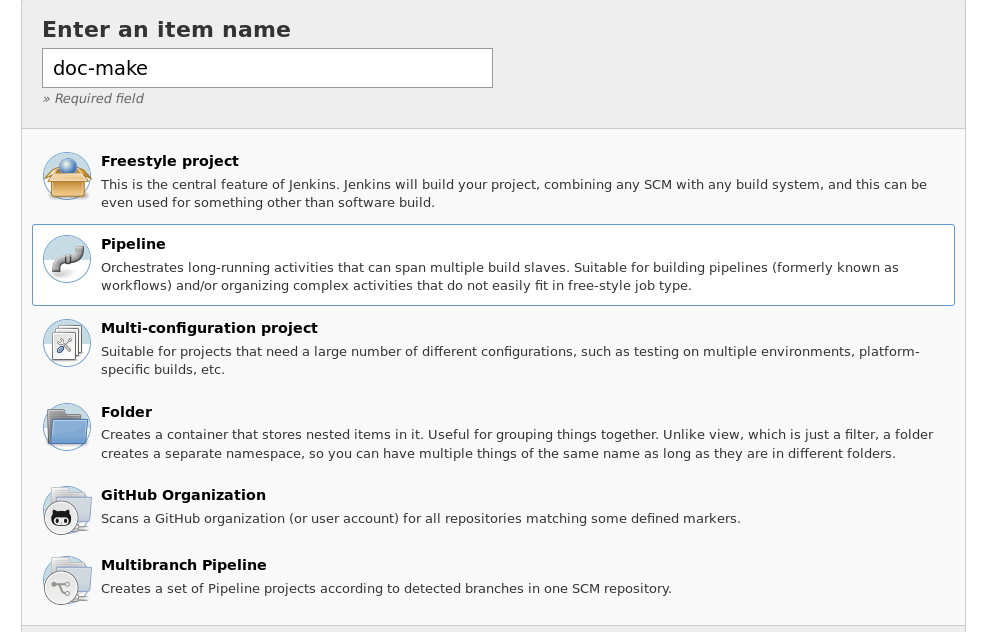
\includegraphics[width=\textwidth,height=0.6\textwidth]{images/jenkins.png}

  \subsection{安裝與基本}
  安裝現在非常簡單,在 https://jenkins.io/download/
  可以用docker 去啟動一個jenkins的docker appliance ,jenkins小組會在docker hub 
  維護 jenkins/jenkins:lts 這個image,只要
  \begin{verbatim}
# docker pull jenkins/jenkins:lts
# docker run -p 8080:8080 -p 50000:50000 jenkins/jenkins:lts
  \end{verbatim}
  或者真的自己裝一個,以我的 debian 來說,只要先裝curl 與 apt-transport-https,然後
  \begin{verbatim}
# curl -fsSL https://pkg.jenkins.io/debian-stable/jenkins.io.key | sudo apt-key add -
  在/etc/source.list加上下面這行
  deb https://pkg.jenkins.io/debian-stable binary
# apt-get update; apt-get install jenkins
  \end{verbatim}
  就完成安裝了。
  \\\\
  安裝完會在8080 port上啟動jenkins,跟CUPS一樣很像,所有的起始與維護都在8080 port
  上開始,一開始會換密碼,加上新使用者,安裝default plugins,就啟動了。
  啟動後又有些新名詞要解釋了,這種management software就是這樣,首先他兩個分類
  \begin{itemize}
    \item JOB/ITEM/PROJECT 就是一個名詞而已,總之create item就只是產生新的build
      project 而已,目前我玩2.89.3的create new item有些template,但其實這些
      template 只是好玩而已,裏面的設定隨時都可以自己亂加進去。
    \item view/my view 其實就是group的意思,每個分類都有大分類,create view 就是
      create 一個大分類項,裏面包含很多job/item/project。list view 是每個人都看
      得到的分類結構,這應該要有權限 , my view 就是自己的整理分類。
  \end{itemize}
  好了現在先create item,目前default 有以下template讓你選並填入project相關資訊
  \begin{itemize}
    \item freestyle 就比較簡單straigforward的tasks資訊輸入。
    \item pipeline 建立pipeline, 這在下面說明。
    \item multi-configuration
    \item folder
    \item github organization 在github上可以建立所謂organization, 就是私人的小組。
      這是跟github溝通用的設定。我記得也有bitbucket的但要額外安裝plugin。
    \item multibranch pipeline 多branch的pipeline
  \end{itemize}
  先選freestyle 最簡單。裏面有GUI設定 git server在哪裡,build跟build間的關係等
  等,然後其實我們很多都只是用build那個步驟的 execute shell 跑我們要的build
  script而已。
  \\\\
  我們還是先看需求
  \begin{itemize}
    \item 整組人員能夠用原本公司內的帳號密碼就login, 這需要LDAP
    \item 管理人員可以有權限設定誰能login誰不能login, 例如公司會計人員就沒必要能
      login
    \item 要能跟source control連結,一但有人trigger build,就能去相關 git/svn 抓
      出相關 branch,啟動一個 build
    \item 要能跟testing report工具連結,一旦測試失敗則這個build也是失敗的。
    \item 要能GUI上debug流程的錯誤在哪。
    \item 能夠發mail, 通知大家結果。
    \item 最好能有pipeline執行不同工作,例如 build, static analysis, automation
      test 等等是可以分開的不同階段的執行,一旦一個完成,別的project可以進入
      pipeline的執行。
    \item build 完後,能在GUI上抓到images。
  \end{itemize}

  \subsection{更多的configuration}
  global system configuration裏面可能 pipeline 是比較新的名詞,其他的就很一般,
  executor就是同時jenkins可以去跑的process數目。
  label就只是別名,可以用這別名來識別操作機器node。
  workspace就是git clone啦,build, testing的目錄,應該是藏在/var/run/jenkins。
  \\\\
  pipeline 就是跟computer architecture上的一樣,完成一件事情需要多階段的tasks,
  從拉出source, build, test到最後deploy到真的機器上,算是生產線流程。
  jenkins管理pipeline,甚至jenkins忽然死掉時,pipeline 的重啟都是自動的。
  pipeline 必須用所謂他的 pipeline dsl語言定義,寫到一個叫Jenkinsfile檔案,
  也有所謂 blue ocean plugin 用GUI輸入參數就幫你輸出一個Jenkinsfile檔案。
  \\\\
  credential configuration 主要是設定其他服務的 uid/password, 像git, slave node
  , email等等服務。 store 與 domain是他分類的大項, 內定store就是master node的
  hostname, 有一個內定 domain 叫 global 是所有的機器都可以用的,自己新創的domain
  裏面可以設定specification, 讓某些機器或設定可以使用而已。就這樣。credential
  的種類有username/password 就是要輸入uid/password的,或者
  ssh Username with private key, 就是使用ssh-keygen產生.ssh/id\_rsa 
  .ssh/id\_rsa.pub 然後把 public key 丟到對方去的,所以輸入是uid/private key,
  ssh-keygen建造時有輸入passphrase,就要輸入jenkins,沒有就沒有。其他方法就是
  有的certificate的方式。certificate說穿了就是public key + 一堆資訊而已。
  \\\\
  manage node, node master 與 slave node 是可以有很多台 build machines 管理,
  其實我很討厭Java, 根本就是resource老饕,所以光裝一台jenkins,很快資源就被吃光
  了,要有其他build machine給他揮霍。剛裝好的jenkins是master node, 主jenkins機器
  ,他可以透過 ssh 控制slave node來完成build, testing 工作,所以我們可
  以在manage node裏面多設幾台 slave node 來讓 master node 來玩他們。說穿了就是
  用 scp 先copy slave.jar 到slave node,然後 ssh 到 slave node 跑slave.jar 而已
  。實際操作時,master node 只是做 conifugraiton 與backup而已,slave node 才是
  真正build, run test的地方,因此 slave node 要先裝好 java,credential
  可以用username/password的方法,但大部分的人是用 privae public key 的方法。
  所以如果是用 root 跑build, copy master node 上 ssh-keygen產生的id\_rsa.pub 到
  slave node 的 /root/.ssh/authorized\_keys, 由於jenkins的內定安裝 Home 是在
  /var/lib/jenkins,所以master node 的 id\_rsa 應該是在/var/lib/jenkins/.ssh 下
  當然如果slave node不是用root跑build job,那就要slave node建立新帳號,把
  id\_rsa.pub放到對的位置。
  \\\\
  create new node選permanent agent, 然後slave node 的remote root directory要改掉
  , 在launch method裏面選"Launch agents via SSH" 然後可以加上creditial後,選他
  就可以了。 至於文件的什麼agent, label就不用去管他了,label只是slave node的別名
  , agent就是那個 ssh 跑起來的session而已。 只是jenkins蠻阿呆的,如果沒有連過
  slave node, .ssh/known\_host沒有slave node資訊,launch agent就會失敗。所以要
  先變身jenkins, 然後 ssh slave node一遍寫進master的known\_host。
  \\\\
  git server的整合,基本git的整合蠻簡單的,這邊是要說明github, bitbucket的整合
  ,我們在前面github, bitbucket時,已經先建立了我們的account,
  \\\\
  user configuration, user 的存取權限

\section{sonarQube}
  sonarQube是個對整體code quality品質統計的一個監督軟體,這通常是經理以上人員
  才有興趣的東西,例如發現為什麼GUI的bugs特別多,或者某方面的分類統計上有異常
  的多或少,根據這些資料來調整組裡的管理事宜。我們公司用這也很多年了,well,
  \href{https://www.sonarqube.org/downloads/}{下載community free版本},也要
  \href{https://openjdk.org/}{下載 openjdk},他也有 container 可以裝,不用
  自己裝這裝那的。
  \begin{itemize}
    \item 解開 openjdk 到 \$HOME/opt/
    \item export JAVA\_HOME=\$HOME/opt/jdk-21.0.2/
    \item export SONAR\_JAVA\_PATH=\$HOME/opt/jdk-21.0.2/bin/java
    \item 啟動 postgreSQL 跟設定 username, password
    \item bin/linux-x86-64/sonar.sh start
    \item http://localhost:9000
    \item 內定uid/passwd : admin/admin
  \end{itemize}
\section{其他}
  共筆wiki與小組文件可以用 wiki.org, readthedocs.org,
  小組文件通常是一些組裡的規定,資訊,例如寫code的convention, lab機器在哪裡
  IP是多少等等,這些可以用wiki的方式讓大家寫作與分享。readthedocs.org是
  另一個文件產生器網站,用rst語法能產生目錄與文件,他是opensource的,所以能
  裝一個到自己內部來使用。
  \\\\
  https://jfrog.com/artifactory/
  \\\\
  artifactory是一個binary release的管理工具。我們公司內部也有用在各組的
  release 管理,這主要用在對內的發佈,正式公司對外發佈有我們的另外一套,
  不過我對binary的管理不是很感興趣,主要是傳統上我們就放在自家file system 
  上就好了,主要是版本,不同images形式,名稱的分門別類然後他是有GUI的就這樣
  , 那公司有可能想要統一中央集權管理這些內部binary release,又我們DE, QA, 
  PM, OPs, Marketing 等組的介面參考,可以很快方便找到,也有人在推用就是。
  \\\\
  https://www.ansible.com/
  \\\\
  ansible是一個自動deploy的工具,但...就是寫個像pipeline定義的檔,
  用的是yml格式,用ssh在一堆遠端執行命令, 通常這些
  工具的好處是有 GUI 操作,統計圖表等等。這種控制非常多台node的程式也叫
  orchestrator, 交響樂的指揮家。傳統上很多公司也都有提供自家的
  orchestration軟體來控管自家的機器,只是現在storage, network等機器都已經
  被opensource virtualization取代,幾乎這些公開的介面已成為標準,所以慢慢
  我想opensource的orchestration軟體最後也會把傳統公司給吃掉的。以前老工程
  師會個私有公司的工具就好像吃不完,現在要熟悉opensource工具組才行。
\section{結語}
  其實由於幾十年來,太多亂七八糟的工具了,所以有人在推,也有很多組用傳
  統的工具,就像code review一樣,我們內部其實從早期自己寫的到review board,
  gerrit, bitbucket, github等一直轉換,現在應該都是 github, bitbucket 了,
  大概也不會再有新工具了。
  \\\\
  不過很多問題的解決不在於使用什麼工具就解決的了,人與人的溝通,衝突,不協
  調問題都在於人的貪嗔痴,這些東西不可能像那些表面所想的用什麼物質,什麼步驟
  就能改變,就能讓大家想的跟你想的一樣,導入什麼工具就萬事ok,如果能,那人就
  不叫人了。一個startup要成功還是要有真正尖端技術,10人以下同心同德專業團隊
  ,做起來後從大眾口袋中拿出一毛錢,賺大錢後才有可能去搞這些大堆頭的管理遊戲
  。
